\label{graph_theory_chapter}
\theoremstyle{plain}
\newtheorem{thm}{Theorem}[chapter] % reset theorem numbering for each chapter
\newtheorem{corollary}{Corollary}[thm]
\newtheorem{lemma}[thm]{Lemma}
\theoremstyle{definition}
\newtheorem{defn}[thm]{Definition}

In this chapter, a brief overview of graph theory will be given. This is not an extensive study of the whole subject, and only the basic definitions and terminology will be presented, especially those that will be useful in the next chapters. This chapter was written such that it could be used as a brief introduction to graph theory to the novices in the subject as well. If the reader has a basic background in graph theory, he can jump to the next chapter.\\
%First, to enter in context and as a motivation, the problem of the seven bridges of Königsberg, which gave %birth to graph theory will be reviewed. 

%\section{A Little Bit of History. The Seven Bridges of Königsberg}
%\label{bridges}
%It is said that in the eighteenth century, in the city of Königsberg in Eastern Prussia, nowadays Kaliningrad, the inhabitants enjoyed taking promenades around town. The city was divided into four parts, two of which were islands surrounded by the river Pregel which divided in two at the central island called Kneiphof. The four parts of the city were connected by seven bridges as can be seen in Fig \ref{fig:konigsberg_city}. While taking walks, the citizens used to discuss and ask themselves if it was possible to find a route which starting in a point then crossed exactly once each bridge to finish in the starting point.

%\begin{figure}
	%\centering
		%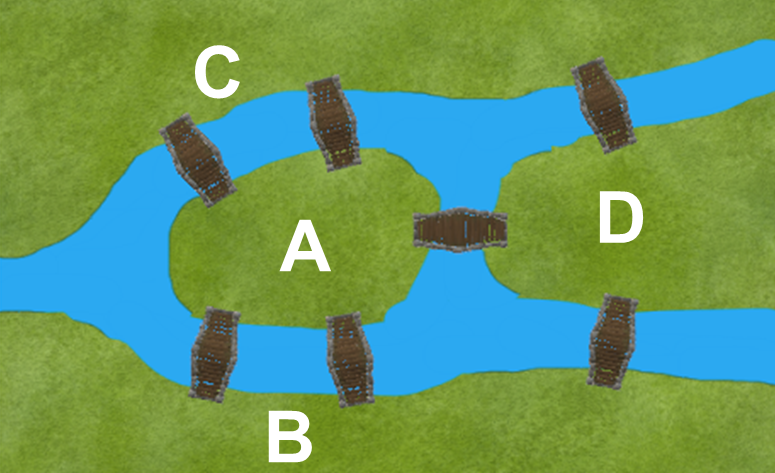
\includegraphics[scale=0.4]{konigsber_city}
	%\caption{The old city of Königsberg.}
	%\label{fig:konigsberg_city}
%\end{figure}

%Some thought that such promenade was impossible, but given the enormous amount of possible paths, it was not possible to prove it until the famous Swiss mathematician Leonard Euler (1707-1783) published a paper which appeared in the 1736 volume of the publications of the Academy of Science in St. Petersburg. In this paper, Euler found a way to prove that such a route was not possible. He simplified the problem by making a clever abstraction of it. He realized that this problem was a new geometric type problem in which no measurements were needed, just the relations between the bridges and the lands were of importance. In fact, although he was not using the modern language of Graph Theory, his technique was implicitly making use of the properties of the graph \footnote{In fact, it is a multigraph which will be defined in \ref{multigraph}.} shown in Fig \ref{fig:konigsberg_graph}. to solve the problem. However, Euler was even beyond and generalized and solved this kind of problems which now are known as finding a Eulerian Trail (or cycle) \cite{harary}.

%\begin{figure}
	%\centering
		%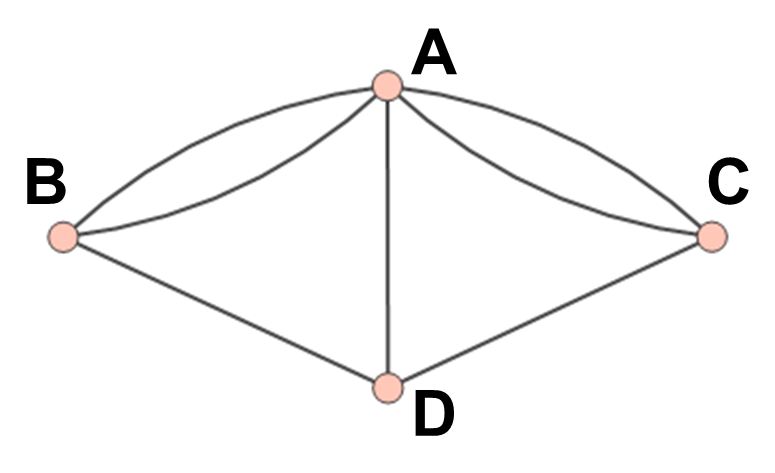
\includegraphics[scale=0.4]{konigsber_graph}
	%\caption{The abstraction of the problem of the seven bridges of Königsberg in the form of a graph made by Euler.}
	%\label{fig:konigsberg_graph}
%\end{figure}

%We will not discuss in more detail the solution of this or related problems because it is out of our reach. In fact, the number of problems and applications of graph theory is so extensive that we would need a complete book in the subject to give a proper introduction in this field of applied mathematics. 


\section{What is a Graph?}
A graph\footnote{Mathematicians prefer the term graph, although some physicists and engineers often refer to them simply as networks. In both cases, they are referring to the same type of object. We will use both terms indistinctly, though the reader should not confuse a Network with the Boolean Networks or Neural Networks which will be studied later.} is defined as follows \cite{douglas}:\\
\begin{defn}
\label{graphdef}
	A \textit{graph G} with \textit{n vertices} and \textit{m edges} consists of a \textit{vertex set} $ V(G)=\{v_{1},...,v_{n}\} $ and an \textit{edge set} $E(G)=\{e_{1},...,e_{m}\} $, where each edge is an unordered pair of vertices. We write $ uv $ for the edge $ \{u,v\} $.\\
\end{defn}

The terminology to refer to the vertices $u$ and $v$ which are the endpoints of an edge $e$ is the following \cite{wilsonwatkins}:\\
\begin{defn}
\label{adjorinc}
If $ uv\in E(G) $, then $ u $ and $ v $ are joined by the edge $e$ and they are said to be \textit{adjacent}. Furthermore, $u$ and $v$ are said to be incident with $e$, and $e$ is said to be incident with $u$ and $v$. 
\end{defn}

There are some special types of edges to be considered and that will help us to classify graphs \cite{wilsonwatkins}:\\

\begin{defn}
	Two or more edges joining the same pair of vertices are called \textit{multiple edges}, and an edge joining a vertex to itself is called a \textit{loop}.\\
\end{defn}

We can classify a graph like simple or not \cite{diestel}:\\

\begin{figure}
	\centering
	\begin{subfigure}[b]{0.4\textwidth}
		\centering
		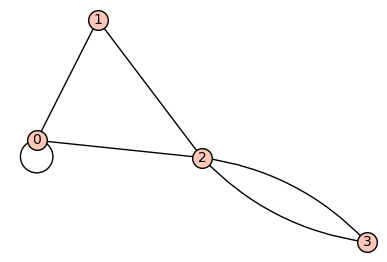
\includegraphics[width=\textwidth]{notsimplegraph}
		\caption{$G_{1}=(V_{1}(G_{1}),E_{1}(G_{1}))$ where\\   $V_{1}=\{0,1,2,3\}$ and\\$E_{1}=\{00,01,02,12,23,32\}$}
		\label{fig:notsimplegraph}
	\end{subfigure}
	\hfill
	\begin{subfigure}[b]{0.4\textwidth}
		\centering
		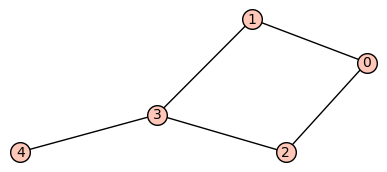
\includegraphics[width=\textwidth]{simplegraph}
		\caption{$G_{2}=(V_{2}(G_{2}),E_{2}(G_{2}))$ where\\   $V_{2}=\{0,1,2,3,4\}$ and\\$E_{2}=\{01,02,13,23,34\}$}
		\label{fig:simplegraph}
	\end{subfigure}
	\caption[A simple graph versus a graph that is not simple.]{(a) The graph $G_{1}$ is not a simple graph because it has a loop and two multiple edges, while in (b) the graph $G_{2}$ is a simple graph.}
	\label{fig:simplevsnotgraph}
\end{figure}

\begin{defn}
	\label{simple}
	A graph with no loops or multiple edges is called a \textit{simple graph}.\\
\end{defn}

\begin{defn}
\label{multigraph}
	A graph with loops or multiple edges is called a \textit{multigraph} \footnote{The term graph indicates the more general case of a multigraph, but often simple graphs are referred just as graphs \cite{douglas}.} \footnote{For some authors, the term multigraph refers to graphs with multiple edges or loops, while for others it refers only to graphs with multiple edges and without loops. See \cite{multigraph}.}.\\
\end{defn}

It is customary to give a visual representation of a graph on paper, drawing a dot for each vertex and a curve or line for each edge joining its endpoints. The previous definitions are illustrated in Fig. \ref{fig:simplevsnotgraph}.\\


The way in that the vertices and edges are drawn or labeled is not relevant, what matters is the information of which pairs of nodes\footnote{Throughout this thesis the words vertex and nodes will be used indistinctly as synonyms.} form an edge and which not \cite{diestel}. Although two graphs may look different, they can be equal (see Fig. \ref{fig:equal}):\\  

\begin{defn}
	\label{equality}
	Two graphs are \textit{equal} if they have equal vertex sets and equal edge sets. And two graph diagrams are \textit{equal} if they represent equal vertex sets and equal edge sets.\\
\end{defn}

\begin{figure}[h]
	\centering
	\begin{subfigure}[b]{0.4\textwidth}
		\centering
		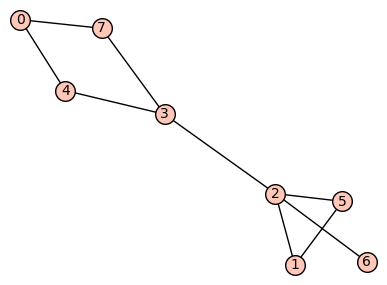
\includegraphics[width=\textwidth]{equalgraph2}
	\end{subfigure}
	\hfill
	\begin{subfigure}[b]{0.3\textwidth}
		\centering
		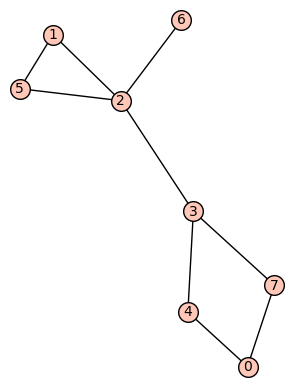
\includegraphics[width=\textwidth]{equalgraph1}
	\end{subfigure}
	\caption{Two graph diagrams that look different but represent the same graph.}
	\label{fig:equal}
\end{figure}

A graph can be "contained" inside another graph. This "smaller" graph is called a subgraph which is defined as follows \cite{trudeau}:\\

\begin{defn}
	A graph $H$ is a \textit{subgraph} of a graph $G$ (written as $H\subseteq G$), if the vertex set of $H$ is a subset of the vertex set of $G$ and the edge set of $H$ is a subset of the edge set of $G$. If $H$ is a subgraph of $G$, it is said that $G$ contains $H$.\\
\end{defn}

It must be noted that a subgraph is another graph and that every graph is a subgraph of itself \cite{wilsonwatkins} (see Fig. \ref{fig:subgraphs}).

\begin{figure}[h]
	\centering
	\begin{subfigure}[b]{0.4\textwidth}
		\centering
		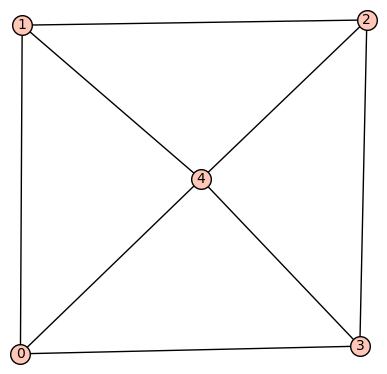
\includegraphics[angle=45,origin=c,width=\textwidth]{subgraph2}
		\caption{$G=(V(G),E(G))$ where\\   $V=\{0,1,2,3,4\}$ and $E=\{01,03,04,12,14,23,24,34\}$}
		\label{fig:subgraph2}
	\end{subfigure}
	\hfill
	\begin{subfigure}[b]{0.4\textwidth}
		\centering
		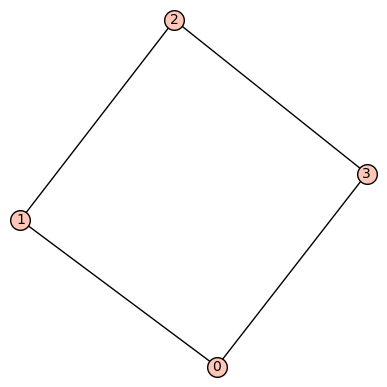
\includegraphics[width=\textwidth]{subgraph1}
		\caption{$H=(V(H),E(H))$ where\\   $V=\{0,1,2,3\}$ and\\$E=\{01,03,12,23\}$}
		\label{fig:subgraph1}
	\end{subfigure}
	\caption[A subgraph.]{(b) is a subgraph of (a).}
	\label{fig:subgraphs}
\end{figure}

\section{The Vertex Degree}
In this section, the basic definitions, used to characterize and describe the number of components of a graph, are given. Then, the handshaking lemma is presented.

\subsection{Some Basic Definitions}
Firstly, it is important to measure how big or small a graph is. The next definitions are helpful for this purpose \cite{douglas}:\\
 
\begin{defn}
	The \textit{order} of a graph $G$, written as $n(G)$ or $|V(G)|$, is the number of vertices in $G$. An \textit{n-vertex graph} is a graph of order $n$.\\
\end{defn}

\begin{defn}
	The \textit{size} of a graph $G$, written as $e(G)$ or $|E(G)|$, is the number of edges in $G$.\\
\end{defn}

When working with graphs it is important to know not only its order or size but also the "number of connections" of each node. This parameter is called the degree of the vertex, and it is defined as \cite{douglas}:\\

\begin{defn}
\label{degree}
	The \textit{degree} of a vertex \textit{v} in a Graph \textit{G}, written $d_{G}(v)$ or $d(v)$, is the number of non-loop edges containing \textit{v} plus twice the number of loops containing \textit{v}.
\end{defn} 

In more simple words, the degree of a vertex is the number of lines connected to it and if the edge is a loop then we count the two connections to it even though they belong to the same edge.\\

A special name is given to the graphs which vertices have the same degree \cite{diestel}:
\begin{defn}
\label{regular}
If all the vertices of \textit{G} have the same degree \textit{k}, then \textit{G} is \textit{k-regular}, or simply \textit{regular}.
\end{defn} 

Examples of regular graphs are shown in Fig. \ref{fig:regular}.

\begin{figure}[h]
	\centering
	\begin{subfigure}[b]{0.4\textwidth}
		\centering
		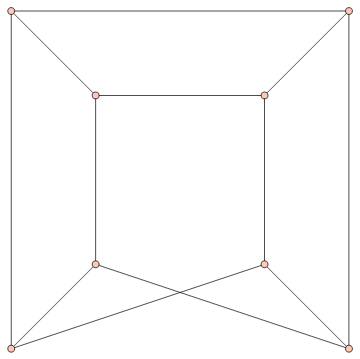
\includegraphics[width=\textwidth]{3regular}
		\caption{A 3-regular graph.}
		\label{fig:regular3}
	\end{subfigure}
	\hfill
	\begin{subfigure}[b]{0.4\textwidth}
		\centering
		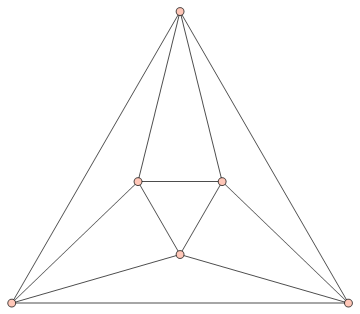
\includegraphics[width=\textwidth]{4regular}
		\caption{A 4-regular graph.}
		\label{fig:regular4}
	\end{subfigure}
	\caption{Examples of regular graphs.}
	\label{fig:regular}
\end{figure}

Unless we are working with regular graphs, the vertices do not need to have the same degree. In such cases, a minimum, and a maximum degree are defined as \cite{diestel}:

\begin{defn}
	The number $\delta(G):=min \{d(v)|v \in V \}$ is the \textit{minimum degree} of \textit{G}, the number $\Delta(G):=max \{d(v)|v \in V \}$ is the \textit{maximum degree}. 
\end{defn} 

If the graphs studied have many nodes, each one most likely having different vertex degree, then it is more convenient to describe the graph by specifying only the average degree of the nodes defined as \cite{diestel}.

\begin{defn}
	The number $d(G):= \frac{1}{|V|} \sum_{v \in V} d(v) $ is the \textit{average degree} of G. The average degree satisfies the relation $\delta(G) \leq d(G) \leq  \Delta(G)$.
\end{defn}

This number quantifies globally the number of edges of \textit{G} per vertex, which is written as $ \varepsilon (G):= \frac{|E|}{|V|}$, and satisfies $ \varepsilon (G)= \frac{1}{2}d(G)$.

\subsection{The Handshaking Lemma}
\begin{lemma}
\label{handshaking}
	\cite{wilsonwatkins}. In any graph \textit{G}, the sum of all the vertex-degrees is equal to twice the number of edges. That is $  \sum d(v)=2|E(G)|$.
\end{lemma}

\begin{corollary}
	\cite{diestel}. The number of vertices of odd degree in a graph is always even.
\end{corollary}

\begin{corollary}
	\cite{wilsonwatkins}. The sum of all the vertex-degrees is an even number.
\end{corollary}

\begin{corollary}
	\cite{wilsonwatkins}. A graph which has n vertices and is r-regular has exactly $ \frac{1}{2} nr$ edges.
	\label{handshaking_corollary}
\end{corollary}

All the concepts presented in this section are summarized in an example in Fig. \ref{fig:definitions}.

\begin{figure}[h]
\centering
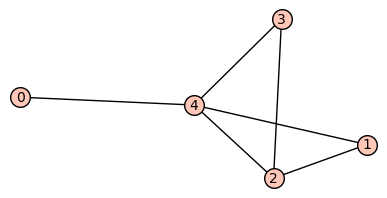
\includegraphics[scale=1]{graphexamplefordefinitions}
\caption[Basic definitions for a graph.]{An example graph $G=(V,E)$ where $V=\{0,1,2,3,4\}$ and $E=\{04,12,14,23,24,34\}$. The order of G is $n(G)=5$. The size of G is $|E(G)|=6$. The degrees of the vertices are: $d(0)=1, d(1)=2, d(2)=3, d(3)=2$ and $d(4)=4$. The handshaking lemma is fulfilled because $1+2+3+2+4=2 \ast 6$; the number of vertices of odd degree is $2$, so its corollary is also fulfilled. The minimum and maximum degrees of $G$ are respectively: $\delta (G)=1$ and $ \Delta (G)=4$. The average degree of $G$ is $d(G)=2.4$ while the number of edges per vertex is $ \varepsilon (G)=1.2$.}
\label{fig:definitions}
\end{figure}

\section{Adjacency and Incidence Matrices}
There are many ways to specify or describe a graph. Until this section, for example, we have been specifying a graph by giving the list of vertices and the list of edges. Nevertheless, in some situations like when we need to generate random graphs or when we want to compute their properties, this can be cumbersome. In such situations, we can rely on more convenient representations using matrices. In this section, we will study the two most common representations of graphs using matrices, although, we must have in mind that they are not the only possible representations. We will continue this discussion in Section \ref{representations}.

\subsection{The Adjacency Matrix}
The adjacency matrix of a graph is built by considering whether the pair of vertices are adjacent or not (see Definition \ref{adjorinc}). For a simple graph, the adjacency matrix is defined as follows \cite{diestel}:

%\begin{defn}
%	The \textit{adjacency matrix} $ A= (a_{ij})_{nxn}$ of a simple graph $G$ is given by:
%		\[a_{ij} = \begin{cases}
%		1 & \text{if $ij \in E$} \\
%		0 & otherwise \\
%		\end{cases}
%		\]
%\end{defn}
\begin{defn}
	The \textit{adjacency matrix} $ A= (a_{ij})_{nxn}$ of a simple graph $G$ is given by:
\begin{equation}		
		a_{ij} = \begin{cases}
		1 & \text{if $ij \in E$} \\
		0 & otherwise \\
		\end{cases}
\end{equation}	
\end{defn}

This definition is generalized for the case of a multigraph \cite{wilsonwatkins}:

\begin{defn}
	The \textit{adjacency matrix} $ A= (a_{ij})_{nxn}$ of a multigraph $G$, is the matrix in which the entry $a_{ij}$ is the number of edges joining the vertices $i$ and $j$. The diagonal entries $a_{ii}$ count the number of loops of the vertex $i$.
		
\end{defn}

The adjacency matrix is symmetric. If it does not have any loops, then it has zeros on the diagonal and the sum of the elements of a column(row) equals the degree of the vertex that the column(row) represents. Furthermore, if the graph is simple, then all its entries are $0's$ or $1's$.\\

%Our definition of the adjacency matrix does not consider graphs with loops if we wish to consider these types of graphs, we must generalize it. To do so, it is helpful to see a property of these matrices: if we sum the values of either a row or a column, then the value we get is equal to the degree of the corresponding vertex. Thus, we can generalize our definition:

%\begin{defn}
%	The \textit{adjacency matrix} $ A= (a_{ij})_{nxn}$ of a graph $G$, is the matrix in which the entry $a_{ij}$ where $i \neq j$, is the number of edges joining the vertices $i$ and $j$. If a vertex $i$ has a loop, then the element of the diagonal $a_{ii}$ equals 2 otherwise equals 0.
		
%\end{defn}

Finally, it must be remarked that a graph may have many adjacency matrices, depending on the way we label and order the vertices.

\subsection{The Incidence Matrix}
Instead of considering the adjacency of the vertices, we can specify a graph by saying if the pairs of vertices are incident or not (see Definition \ref{adjorinc}). The incidence matrix is defined as follows \cite{diestel}: 

%\begin{defn}
%	The \textit{incidence matrix} $ B= (b_{ij})_{nxm}$ of a simple graph $G$ with $n$ vertices and $m$ edges is given by:
%		\[b_{ij} = \begin{cases}
%		1 & \text{if $v_{i} \in e_{j}$} \\
%		0 & otherwise \\
%		\end{cases}
%		\]
%\end{defn}
\begin{defn}
	The \textit{incidence matrix} $ B= (b_{ij})_{nxm}$ of a simple graph $G$ with $n$ vertices and $m$ edges is given by:
\begin{equation}
		b_{ij} = \begin{cases}
		1 & \text{if $v_{i} \in e_{j}$} \\
		0 & otherwise \\
		\end{cases}
\end{equation}
\end{defn}

If we wish to consider multigraphs with loops, then we will generalize this definition as:

%\begin{defn}
%	The \textit{incidence matrix} $ B= (b_{ij})_{nxm}$ of a multigraph $G$ with $n$ vertices and $m$ edges is given by:
%		\[b_{ij} = \begin{cases}
%		1 & \text{if $v_{i} \in e_{j}$} \\
%		2 & \text{if $v_{i}$ is doubly incident with the loop $e_{j}$} \\
%		0 & otherwise \\
%		\end{cases}
%		\]
%\end{defn}
\begin{defn}
	The \textit{incidence matrix} $ B= (b_{ij})_{nxm}$ of a multigraph $G$ with $n$ vertices and $m$ edges is given by:
\begin{equation}
		b_{ij} = \begin{cases}
		1 & \text{if $v_{i} \in e_{j}$} \\
		2 & \text{if $v_{i}$ is doubly incident with the loop $e_{j}$} \\
		0 & otherwise \\
		\end{cases}
\end{equation}
\end{defn}


As in the case of the adjacency matrix, the incidence matrix also depends on the way the edges and vertices are labeled. Some examples of the adjacency and incidence matrices of three different graphs are shown in Fig. \ref{fig:adjinc}.

\begin{figure}
	\centering
	\begin{subfigure}[b]{0.3\textwidth}
		\centering
		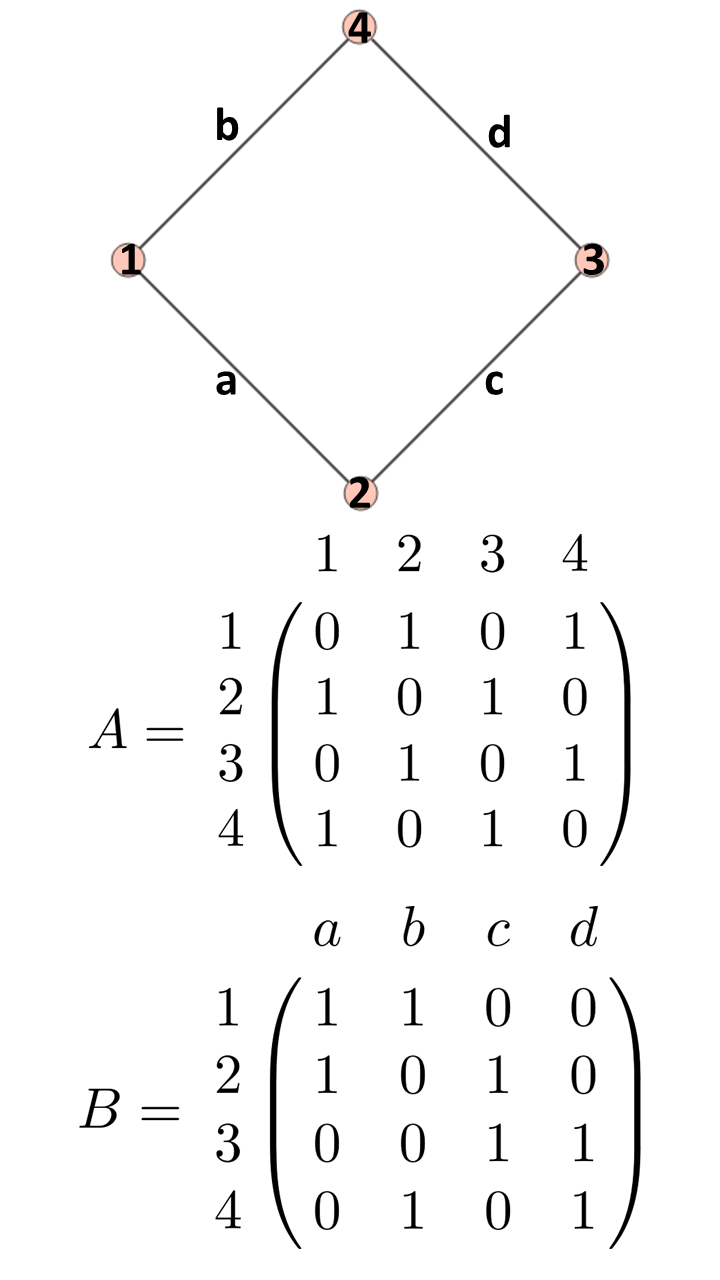
\includegraphics[width=\textwidth]{adjinc1}
		\caption{}
		\label{fig:adjinc1}
	\end{subfigure}
	\hfill
	\begin{subfigure}[b]{0.3\textwidth}
		\centering
		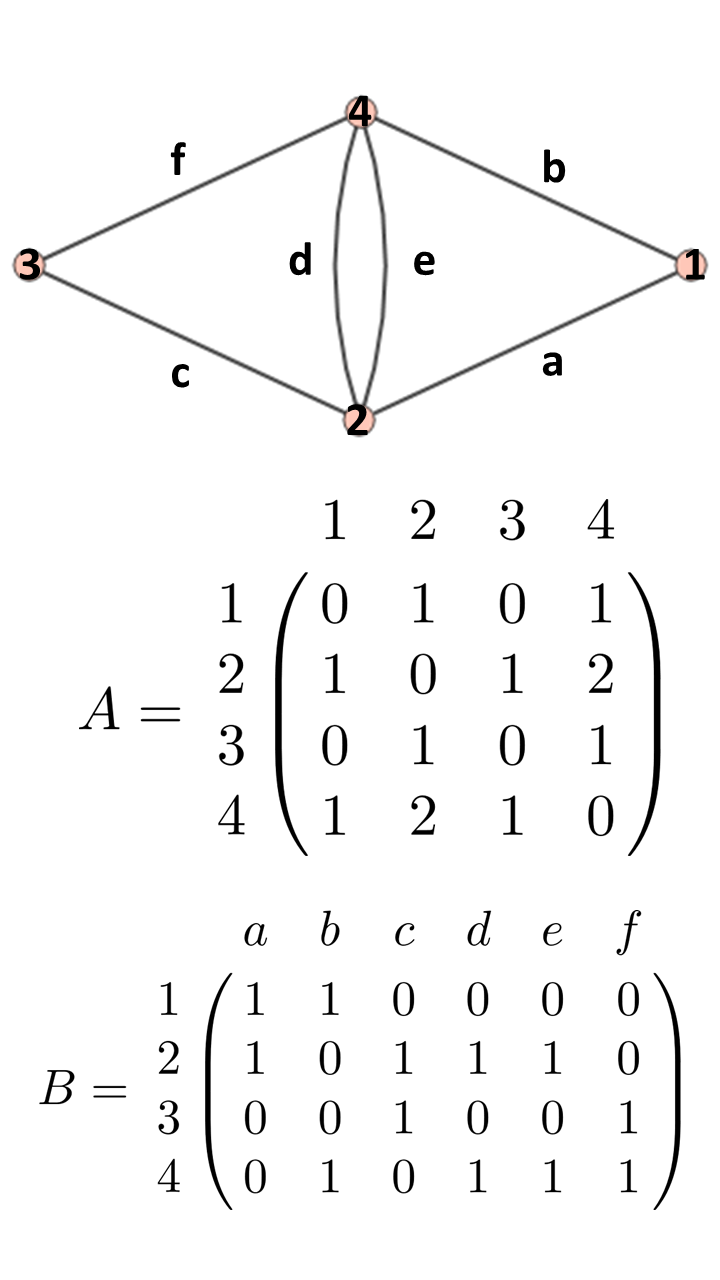
\includegraphics[width=\textwidth]{adjinc2}
		\caption{}
		\label{fig:adjinc2}
	\end{subfigure}
	\begin{subfigure}[b]{0.3\textwidth}
		\centering
		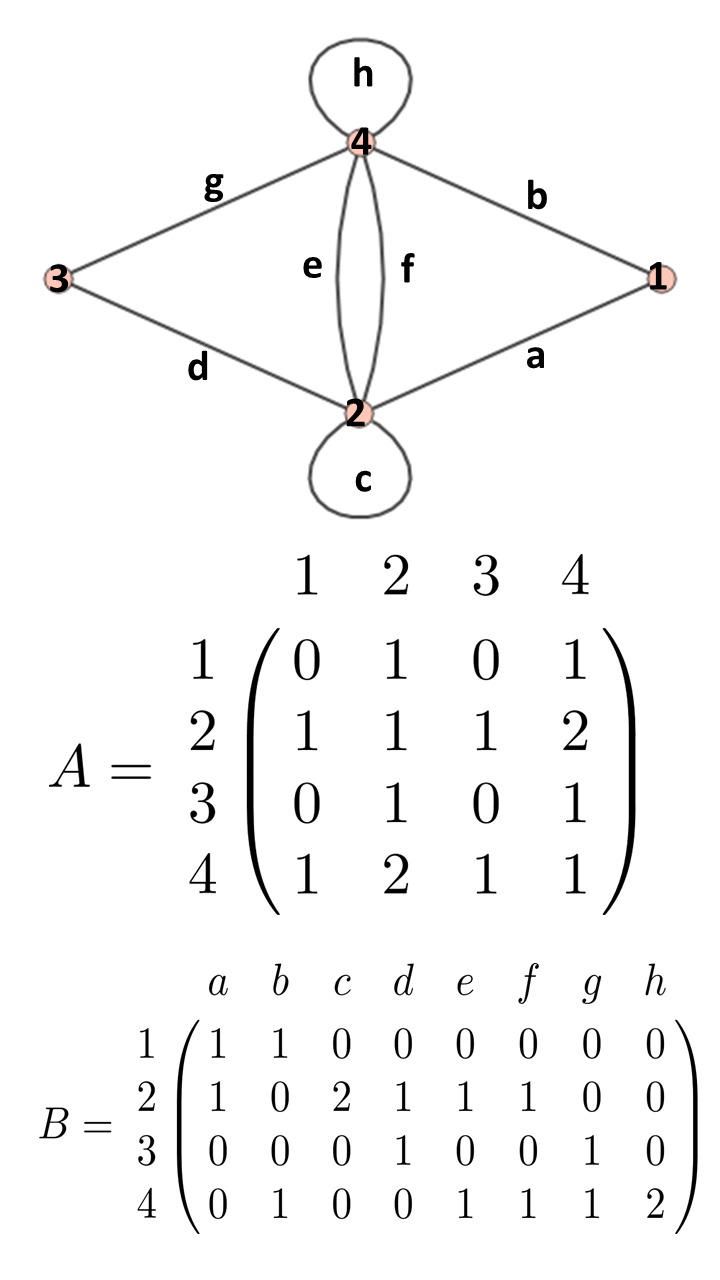
\includegraphics[width=\textwidth]{adjinc3}
		\caption{}
		\label{fig:adjinc3}
	\end{subfigure}
	\caption[Adjacency and incidence matrices.]{Three different graphs with their respective \textit{adjacency matrix} $A$ and \textit{incidence matrix} $B$. (a) A simple Graph. (b) A multigraph without loops. (c) A multigraph with two loops.}
	\label{fig:adjinc}
\end{figure}

\section{Isomorphic Graphs}
\label{isomorphic}
In Definition \ref{equality}, we had a first approach to the equality of 
graphs. However, if we consider two graphs which only differ in the way 
their vertex sets have been labeled, then our definition is not able to 
capture that kind of "sameness" (see Fig. \ref{fig:isomorphic} ) \cite{trudeau}. For such 
situations, we ought to have a suitable definition that does not depend 
on the name of the vertices \cite{diestel}.

\begin{defn}
        Let $G=(V,E)$ and $G'=(V',E')$ be two graphs. We call $G$ and $G'$ 
\textit{isomorphic}, and write $G \cong G'$, if there exists a bijection 
$f: V \rightarrow V'$ with $xy\in E$ $\Leftrightarrow$ $f(x)f(y) \in E'$ 
for all $x,y \in V$. Such a map $f$ is called an \textit{isomorphism}\footnote{The reader must not confuse the concepts of isomorphism and isomorphic. Isomorphism refers to a bijection $f$ while isomorphic refers to an object $G'$ which can be obtained by applying such bijection $f$ to an object $G$.}; 
furthermore, if $G=G'$, it is called an \textit{automorphism}. We do not normally 
distinguish between isomorphic graphs. Thus, we usually write $G=G'$ 
rather than $G \cong G'$.
\end{defn}

Thus, we can say that an isomorphic graph $G'$ can be obtained from $G$ by relabeling its vertices in such a way that there is a one-to-one correspondence between the vertices of $G$ and $G'$ such that the number of edges joining each pair of vertices in $G$ is preserved for the corresponding pair of vertices in $G'$. Therefore, an easy way to construct isomorphic graphs of a graph $G$, is just using permutation matrices to permute the rows and columns of its adjacency matrix $A(G)$  to get an adjacency matrix corresponding to a graph $G'$ which only differs from $G$ in the order we have labeled the vertices. Evidently, isomorphic graphs present transitivity, that is, if $G \cong G'$ and $G' \cong G''$ then $G \cong G''$.

The collection of isomorphisms $f$ of a graph $G$ which are also automorphisms (graph isomorphisms with themselves) form a group called the automorphism group and denoted as $Aut(G)$. This automorphism group preserves the incidence matrix of $G$, i.e., the incidence matrix is an invariant of this group \cite{automorphism}.

\begin{figure}
	\centering
	\begin{subfigure}[b]{0.8\textwidth}
		\centering
		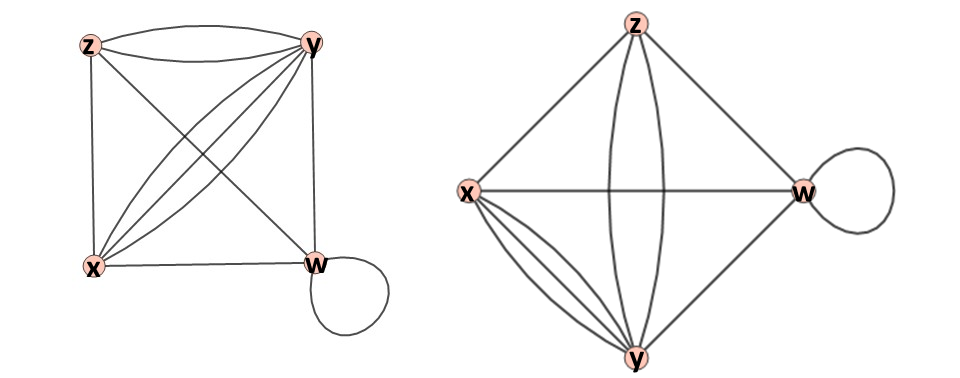
\includegraphics[width=\textwidth]{isomorphism1}
		\caption{}
		\label{fig:iso1}
	\end{subfigure}
	\hfill
	\begin{subfigure}[b]{0.8\textwidth}
		\centering
		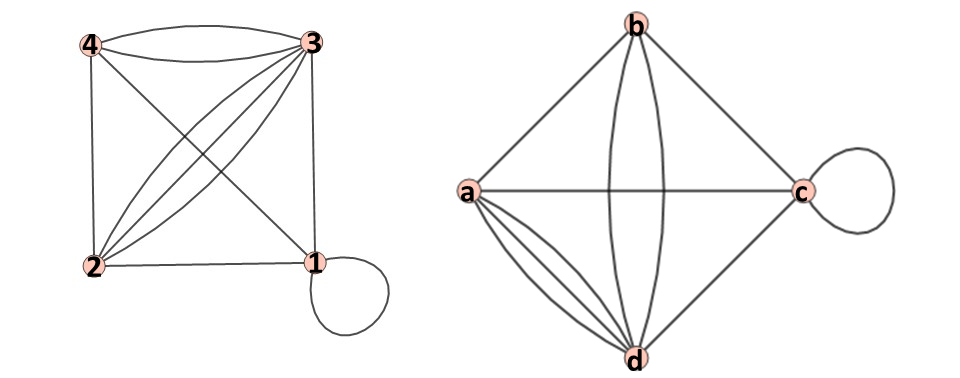
\includegraphics[width=\textwidth]{isomorphism2}
		\caption{}
		\label{fig:iso2}
	\end{subfigure}
	\begin{subfigure}[b]{0.8\textwidth}
		\centering
		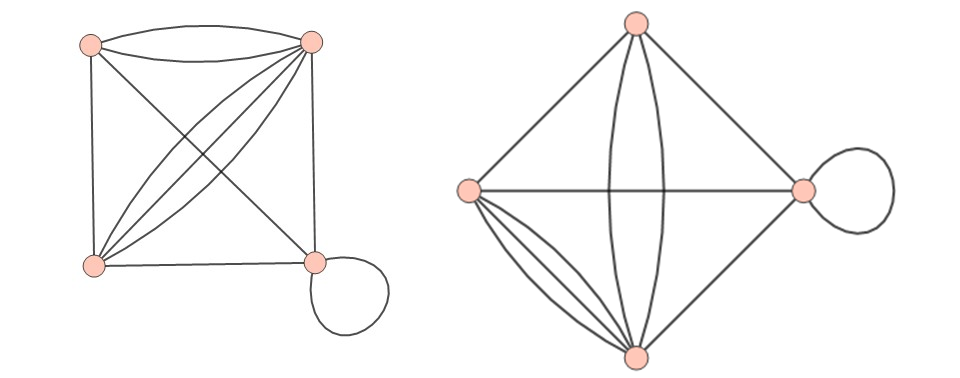
\includegraphics[width=\textwidth]{isomorphism3}
		\caption{}
		\label{fig:iso3}
	\end{subfigure}
	\caption[Isomorphic graphs.]{(a) Labeled graphs that are the same. (b) Labeled graphs that are not the same but are isomorphic. (c) Unlabeled graphs that are isomorphic (they are not labeled to highlight the fact that they are isomorphic independently of the labels chosen).}
	\label{fig:isomorphic}
\end{figure}

\section{Paths and Cycles}
%As was seen in section \ref{bridges}, the Königsberg Bridge Problem gave birth to graph theory. In this problem, Leonhard Euler tried to figure out if there was possible to cross each bridge just once and return to home. This type of \textit{pathway problems} are frequent in graph theory. 

Firstly, we define what we understand when we talk about a \textit{walk} \cite{wilsonwatkins}:

\begin{defn}
        A \textit{walk of length k} in a graph \textit{G} is a succession of \textit{k} edges of \textit{G} of the form \textit{ab, bc, cd, ..., ef}. We denote this walk by \textit{abcd...ef} and refer to it as a \textit{walk between a and f}. \footnote{Since in simple graphs the direction of the edges is not specified, we could refer to this walk as a \textit{walk between f and a}.}
\end{defn}

This definition allows the repetition of edges and vertices. A particular type of walk is a trail, and a particular case of a trail is a path. We define them as follows \cite{wilsonwatkins}:

\begin{defn}
        If all the edges (but not necessarily all the vertices) of a walk are different, then the walk is called a 
        \textit{trial}. If, in addition, all the vertices are different, then the trail is called a \textit{path}.
\end{defn}

Now, we will define the case when the walk has the restriction that it starts and finishes at the same vertex \cite{wilsonwatkins}:
%In the problem of the seven bridges of Königsberg, Euler was interested in finding a walk with the restriction that the start and the finish were at the same vertex. We need to define such types of walks or trials \cite{wilsonwatkins}:

\begin{defn}
\label{closed_walk}
        \textit{A closed walk} in a graph \textit{G} is a succession of edges of \textit{G} of the form \textit{ab, bc, cd, ..., ef,fa}. If all those edges are different, then the walk is called a \textit{closed trail}. If, in addition, the vertices \textit{a,b,c,d,...,e,f} are all different, then the trail is called a cycle. 
\end{defn}

In closed walks, the vertex of beginning can be anyone. An example of a walk is shown in Fig. \ref{fig:walk_path}.\\

\begin{figure}
	\centering
		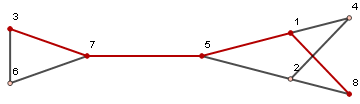
\includegraphics[scale=0.8]{walk}
	\caption[Example of a walk.]{A walk of length $4$ between vertices $3$ and $8$. All the edges are different, so we can consider this walk as a trail. Furthermore, all the vertices are different so we can consider it as a path.}
	\label{fig:walk_path}
\end{figure}

Using the concept of path, we can define a new class of graph \textit{G}, which have the particularity that any two of its vertices are \textit{connected} by a path \cite{wilsonwatkins}:

\begin{defn}
\label{connected}
        A graph \textit{G} is \textit{connected} if there is a path in \textit{G} between any given pair of vertices, and \textit{disconnected} otherwise. Every disconnected graph can be split up into several connected subgraphs, called \textit{components}.
\end{defn}

In Fig. \ref{fig:connect}, examples of connected and disconnected graphs are shown.

\begin{figure}[h]
	\centering
	\begin{subfigure}[b]{0.4\textwidth}
		\centering
		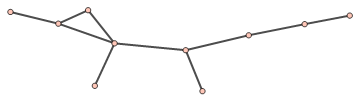
\includegraphics[width=\textwidth]{connected}
		\caption{A connected graph.}
		\label{fig:regular3}
	\end{subfigure}
	\hfill
	\begin{subfigure}[b]{0.4\textwidth}
		\centering
		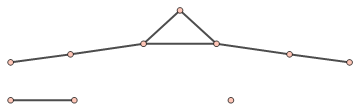
\includegraphics[width=\textwidth]{disconnected}
		\caption{A disconnected graph.}
		\label{fig:regular4}
	\end{subfigure}
	\caption{Examples of connected and disconnected graphs.}
	\label{fig:connect}
\end{figure}

\section{Some Families of Graphs}
There exist many families and ways to classify graphs based on different properties, like the number or degree of the vertices, symmetries, etc. Even there are graphs so interesting that they can have their own special name. Indeed, we have already found some families of graphs in definitions \ref{regular} and \ref{connected}.\\

For the sake of completeness, in this section, a few of the most important families of graphs will be presented. Although we will have to leave out of discussion some families as the \textit{Platonic graphs}, \textit{the planar graphs} or the \textit{Petersen graph}, a complete reference about the names and families of graphs can be found in the literature compiled by the Documentation Center of the Wolfram Language \& System in \cite{graphfamilies} or in the references given at the end of this thesis.

\subsection{Null Graphs}
The \textit{null graph} on \textit{n} vertices, denoted as $N_{n}$, is the graph which has the vertex set $V= \{v_{1},v_{2},v_{3},...,v_{n} \}$ and no edges \cite{trudeau}. Obviously, $N_{n}$ is zero regular. The first six null graphs are shown in Fig. \ref{fig:null_graph}.

\begin{figure}
	\centering
		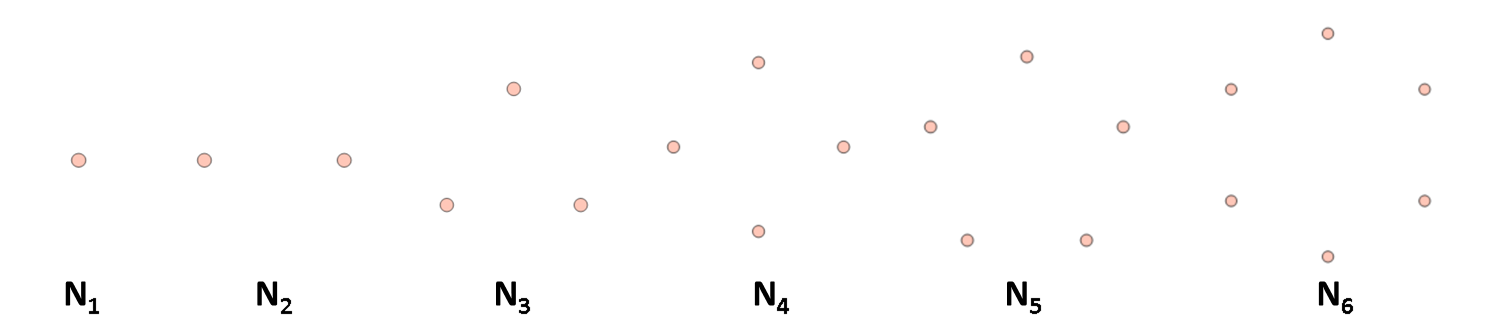
\includegraphics[width=\textwidth]{null_graph}
	\caption{The first six null graphs.}
	\label{fig:null_graph}
\end{figure}

\subsection{Complete Graphs}
A more interesting family is the family of complete graphs. A \textit{complete graph}  on \textit{n} vertices, denoted as $K_{n}$, is the graph having vertex set $V=\{v_{1},v_{2},v_{3},...,v_{n}\}$ and all possible edges, i.e., every two distinct vertices are joined exactly by one edge \cite{trudeau}. The complete graph $K_{n}$ is $(n-1)$-regular and has $\frac{1}{2} n(n-1)$ edges, following the handshaking lemma in \ref{handshaking}. The first six complete graphs are shown in Fig. \ref{fig:complete_graph}.

\begin{figure}
	\centering
		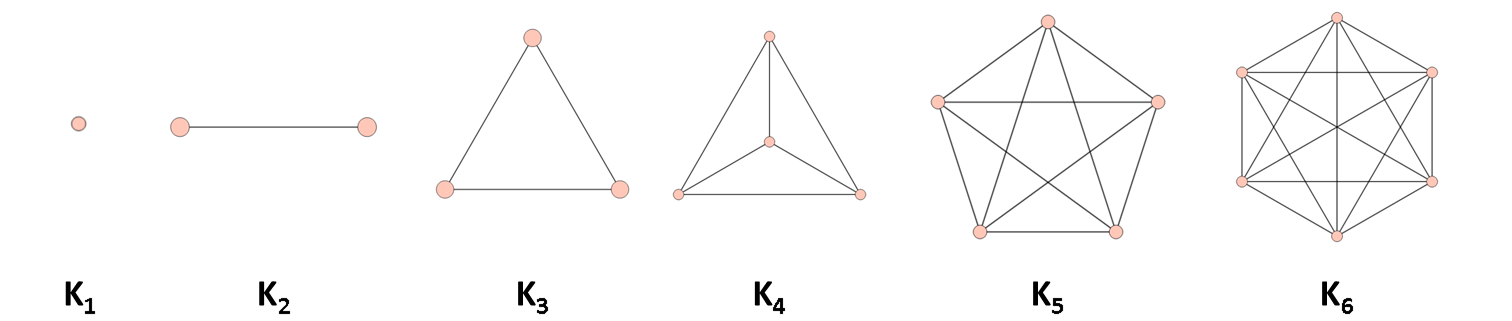
\includegraphics[width=\textwidth]{complete_graph}
	\caption{The first six complete graphs.}
	\label{fig:complete_graph}
\end{figure}

\subsection{Cycle Graphs}
The \textit{cycle graph} or \textit{cyclic graph} on \textit{n} vertices, denoted as $C_{n}$, is the graph consisting of a single cycle (see Definition \ref{closed_walk}). It has the vertex set $V= \{ v_{1},v_{2},v_{3},...,v_{n} \}$ and the edge set $E= \{ v_{i}v_{i+1} | i=1,...n-1 \} \bigcup \{v_{1} v_{n} \}$. \footnote{For some authors, an additional requirement when defining the \textit{cycle graph} on \textit{n} vertices is that \textit{n} must be equal or greater than \textit{3}.}
The cycle graph $C_{n}$ has \textit{n} edges and is 2-regular \cite{wilsonwatkins}. The first six cycle graphs are shown in Fig. \ref{fig:cycle_graph}.

\begin{figure}
	\centering
		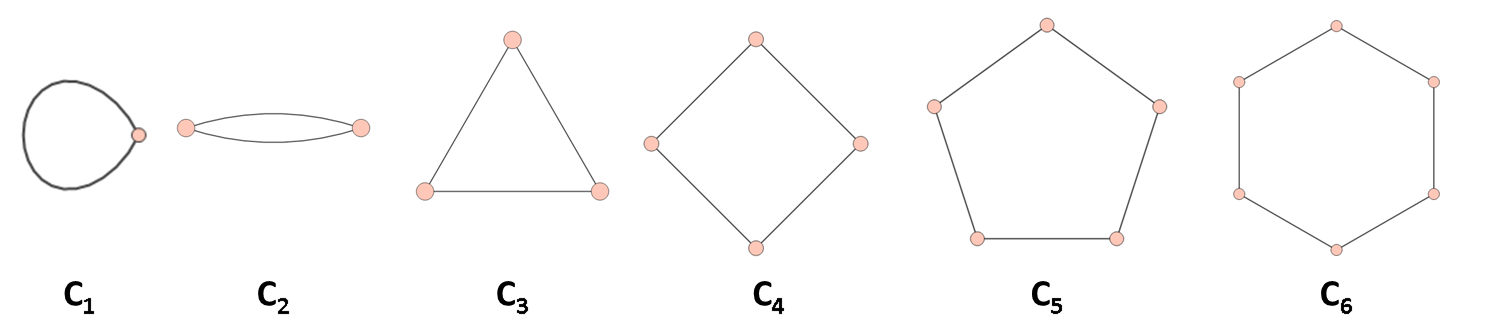
\includegraphics[width=\textwidth]{cycle_graph}
	\caption{The first six cycle graphs.}
	\label{fig:cycle_graph}
\end{figure}

\subsection{Path Graphs}
This family as the name indicates is the family which graphs consist of only a single path. A \textit{path graph}  on \textit{n} vertices, denoted as $P_{n}$, is the graph which has the vertex set $V= \{ v_{1},v_{2},v_{3},...,v_{n} \}$ arranged in a sequence  such that the edge set is  $E= \{ v_{i}v_{i+1} | i=1,...n-1 \} $. We can obtain the path graph $P_{n}$ which has $n-1$ edges, from the cycle graph $C_{n}$ by removing any edge \cite{wilsonwatkins}. The first six path graphs are shown in Fig. \ref{fig:path_graph}.

\begin{figure}
	\centering
		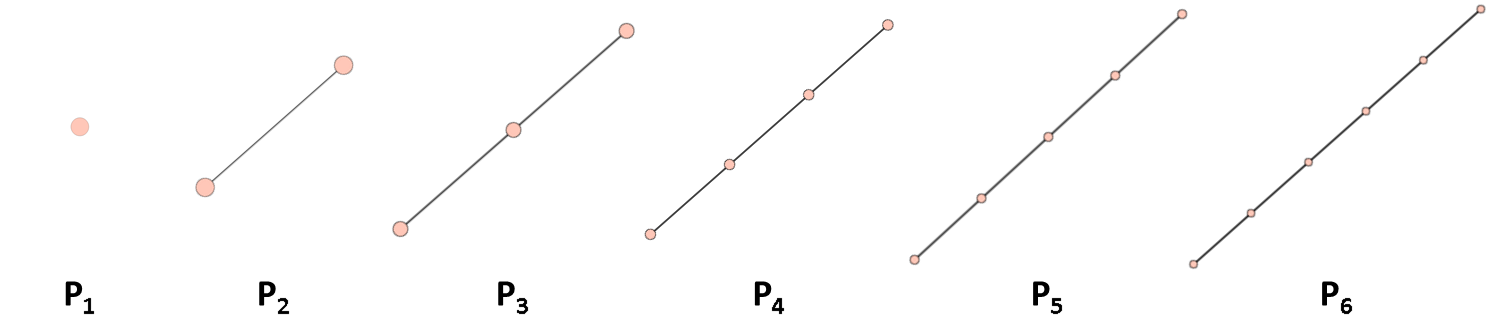
\includegraphics[width=\textwidth]{path_graph}
	\caption{The first six path graphs.}
	\label{fig:path_graph}
\end{figure}

\subsection{Bipartite Graphs}
In this family, we found the graphs whose vertex set $V$ admits a partition into two classes $V_{1}$ and $V_{2}$ such that every edge $uv \in E$ joins a vertex in $V_{1}$ to a vertex in $V_{2}$, i.e., $u \in V_{1}$ and $v \in V_{2}$. Two examples of bipartite graphs are shown in Fig. \ref{fig:bipartite_graph}.

\begin{figure}
	\centering
		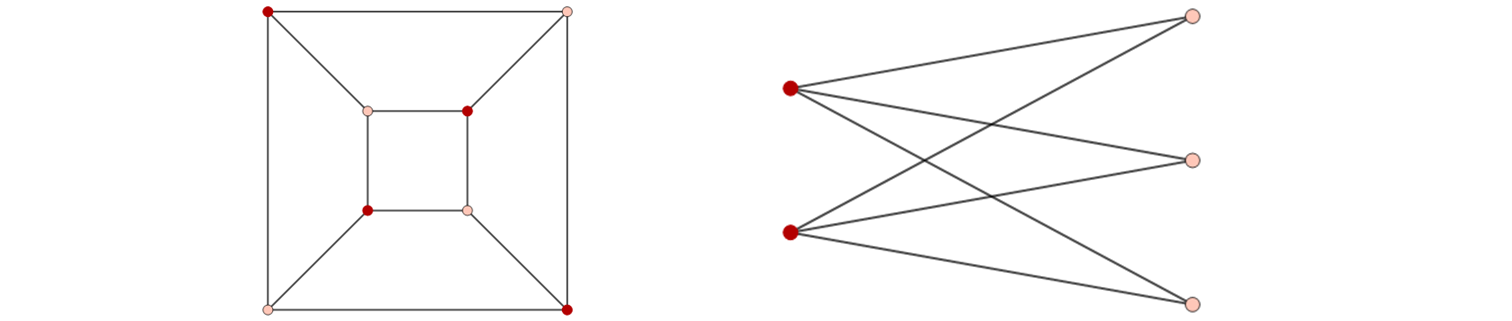
\includegraphics[width=\textwidth]{bipartite_graph}
	\caption[Two examples of bipartite graphs.]{Two examples of bipartite graphs. As can be seen, the vertex sets of both graphs have been divided into two sets (of a different color) in such a way that they satisfy the definition of a bipartite graph.}
	\label{fig:bipartite_graph}
\end{figure}

Furthermore, the \textit{complete bipartite graph}, denoted as $K_{n,m}$, is the bipartite graph in which each vertex in $V_{1}$ is joined to each vertex in $V_{2}$ by exactly one edge, where $|V_{1}|=n$ and $|V_{2}|=m$. The special case $K_{1,m}$ is called a \textit{star graph} \cite{diestel}.

The graph $K_{n,m}$ has $n+m$ vertices (where $n$ are of degree $m$ and $m$ are of degree $n$) and $nm$ edges. Finally, it must be noted that $K_{n,m}=K_{m,n}$, so we usually put the smaller number in the first index \cite{wilsonwatkins}. Some examples of complete bipartite graphs are shown in \ref{fig:complete_bipartite_graph}.

\begin{figure}
	\centering
		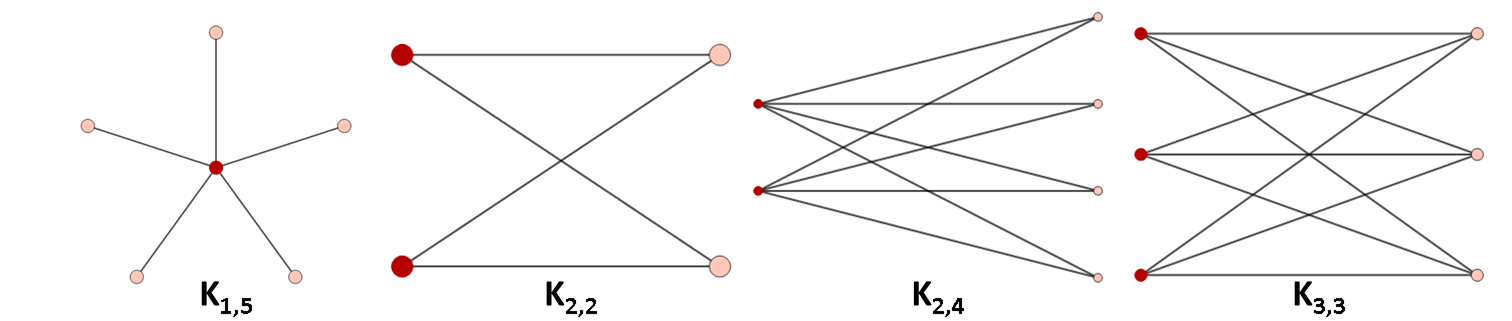
\includegraphics[width=\textwidth]{complete_bipartite_graph}
	\caption[Examples of complete bipartite graphs.]{Examples of complete bipartite graphs. The first graph on the left is also a star graph.}
	\label{fig:complete_bipartite_graph}
\end{figure}

\subsection{Cube Graphs}
The \textit{n-cube graph}, also known as \textit{n-hypercube graph} and denoted as $Q_{n}$, is the graph whose vertices are the $2^{n}$ possible binary words (sequences of $0's$ and $1's$) of length $n$ of which two vertices are adjacent (are joined) if the two corresponding binary words are the same except for one element \cite{hypercube}.
We note that $Q_{n}$ has $n \cdot 2^{n-1}$ edges following the handshaking lemma \ref{handshaking}.
This type of graphs has applications in coding theory \cite{wilsonwatkins}.
The first four cube graphs are shown in Fig. \ref{fig:cube_graph}.

\begin{figure}
	\centering
		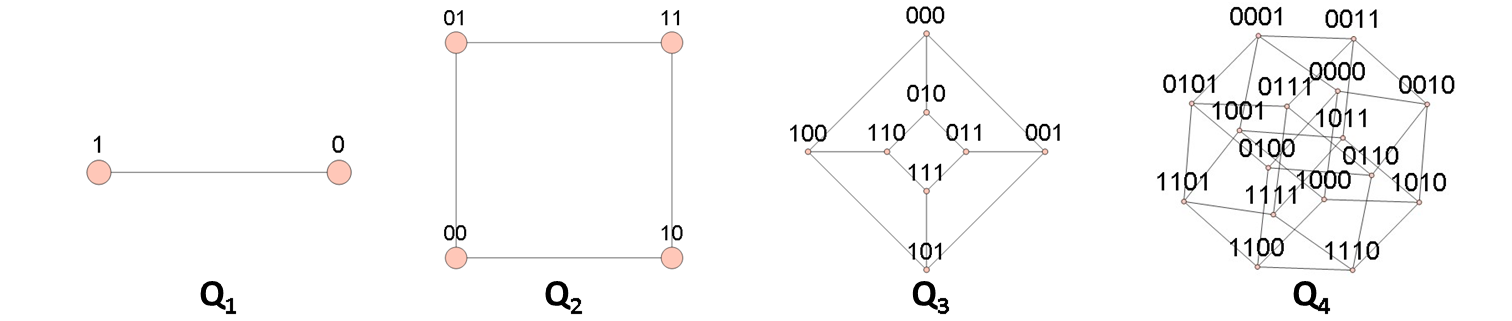
\includegraphics[width=\textwidth]{cube_graph}
	\caption{The first four cube graphs.}
	\label{fig:cube_graph}
\end{figure}

\subsection{Trees}
\label{trees}
If a graph does not have any cycles or circuits (see Definition \ref{closed_walk}), it is called a \textit{forest}. If a \textit{forest} is connected (see Definition \ref{connected}), then it is a \textit{tree}, or in other words: A \textit{tree} is a connected graph which is acyclic, and a forest is a graph whose components are trees, as shown in Fig. \ref{fig:tree_graph}. This definition means that in a tree we found no multiple edges and that there is a unique arc or branch connecting any pair of vertices. Following the analogy, the vertices of degree 1 in a tree are called leaves \cite{diestel}. A tree with $n$ vertices has $n-1$ edges \cite{oystein}.

Let \textit{G} be a connected graph, then we define a \textit{spanning tree in G} as a subgraph of \textit{G} which includes every vertex in \textit{G} and which is also acyclic \cite{wilsonwatkins}. An example of a \textit{spanning tree} is shown in Fig. \ref{fig:spanning_tree_graph}.

\textit{Trees} have many applications in computer science, especially in data storage and communication. For instance, these graphs are used in the Huffman coding, a type of coding that is used for lossless data compression and that is part of the algorithm used in the ZIP compression method \cite{douglas}. Another application is the k-dimensional tree, a type of space-partitioning data structure for organizing information which then can be used to access data in a more efficient way in algorithms of search such as the algorithm of the k-nearest neighbors which is used in machine learning or the depth-first search (DFS) and the breadth-first search (BFS) which are used when a particular piece of information in the random-access memory (RAM) of a computer file is needed \cite{wilsonwatkins}.


\begin{figure}
	\centering
		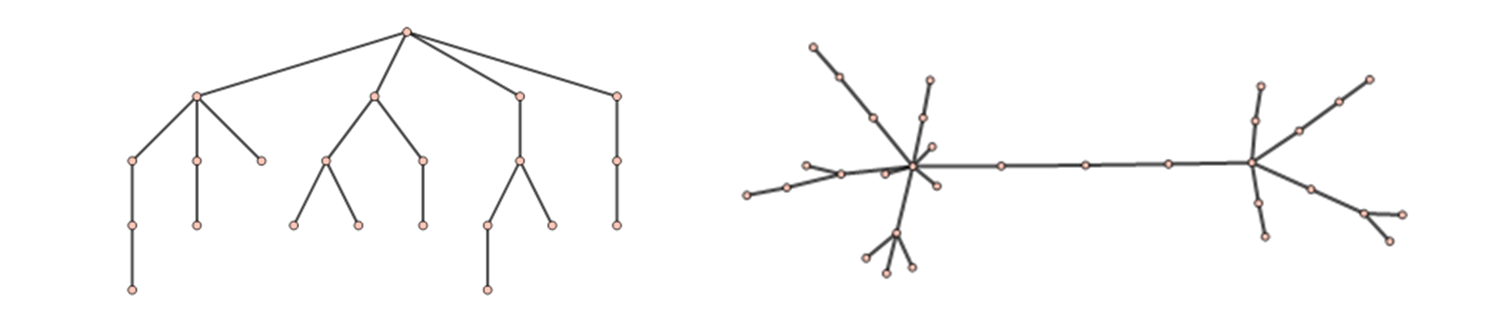
\includegraphics[width=\textwidth]{tree_graph}
	\caption{Two examples of tree graphs.}
	\label{fig:tree_graph}
\end{figure}

\begin{figure}
	\centering
		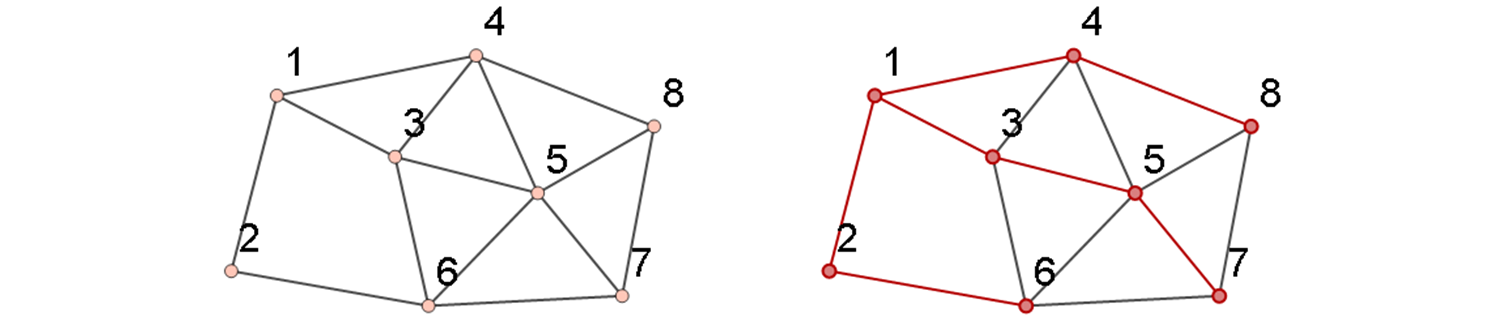
\includegraphics[width=\textwidth]{spanning_tree_graph}
	\caption[An example of a spanning tree.]{On the left, we can see a connected graph and on the right one of its subgraphs (highlighted) which is a spanning tree.}
	\label{fig:spanning_tree_graph}
\end{figure}

\subsection{Circulant Graphs}
These graphs are defined as follows \cite{circulant}:

\begin{defn}
	A \textit{circulant graph} is a graph of $n$ vertices in which the $i$th graph vertex is adjacent to the $(i+j)$th and $(i-j)$th graph vertices for each $j$ in a list of jumps $\{j_{1},j_{2},...\}$. The circulant graph $Ci_{n} (1,2,...,\lfloor n/2 \rfloor)$ is equal to the complete graph $K_{n}$ and the graph $Ci_{n}(1)$ gives the cyclic graph $C_{n}$.
\end{defn}

Some examples of these types of graphs are shown in Fig. \ref{fig:circulant}.

\begin{figure}
	\centering
		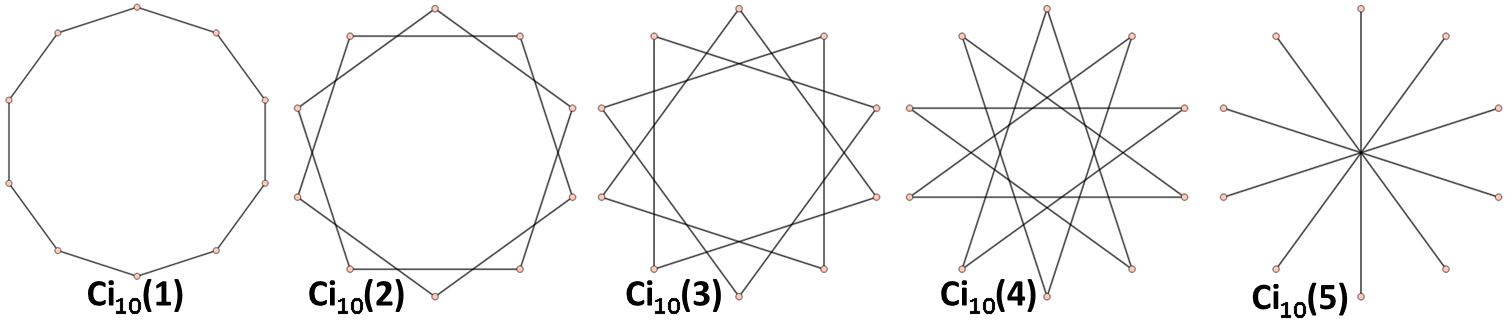
\includegraphics[width=\textwidth]{circulant}
	\caption[Circulant graphs.]{Circulant graphs of $10$ vertices and only one jump. The jumps are $1,2,3,4,$ and $5$ respectively.}
	\label{fig:circulant}
\end{figure}

\section{Counting Graphs}
A natural question arises when generating graphs with certain given properties: how many different graphs of a certain kind there exist? For instance, we could ask: How many different graphs of a given number of vertices there exist? We would find that in general, the number of possible graphs with some given characteristics increases fast with the number of vertices and that in certain situations the problem to find this number is yet open \cite{wilsonwatkins}. To illustrate it, let us see what happens with two of the simplest cases.

\subsection{Labeled Graphs}
\label{count}
We will consider labeled simple graphs which are not isomorphic, so we say that we are counting up to isomorphism. The problem is to find the number of this kind of graphs given the number $n$ of vertices. If we first take into account the $(n-1)$-regular graph of $n$ vertices which has all the possible edges for the type of graphs we are considering, thus by means of the corollary \ref{handshaking_corollary} it has $ \frac{1}{2} n(n-1)$ edges. The rest of the graphs will have or not each of these edges (there are two possibilities), then the number of possible graphs is $ 2^{ \frac{1}{2} n(n-1) }$. For instance, for $n=4$ the number of labeled graphs is $64$, while for $n=7$ the number increases up to $2097152$.

\subsection{Unlabeled Graphs}
Here, we treat with non-isomorphic unlabeled graphs. This problem is not as easy to solve as it was for labeled graphs. Usually, we will have to invoke formulas (if they exist) as the general formula found by George Pólya in 1935 to count graphs with any number of vertices and edges \cite{wilsonwatkins}. As a reference we can see the Table \ref{tab:unlabeled_graphs}, which also contains the number of unlabeled connected graphs and unlabeled regular graphs up to $8$ vertices, and presents the same behavior stated previously, the number of graphs increases fast with the number of vertices $n$.\\

As stated before, there exist formulas like the general formula of George Pólya to count other types of graphs. An example is the Caley's Theorem which states that the number of labeled trees with $n$ vertices is $ n^{n-2}$. However, this is not always the case and sometimes the problem remains unsolved for both labeled and unlabeled graphs or just for one of these cases. In general counting problems for labeled graphs are much easier to solve \cite{wilsonwatkins}.

\begin{table}[t]
\centering
\begin{tabular}{ |c|c|c|c|c|c|c|c|c| } 
 \hline
 n & 1 & 2 & 3 & 4 & 5 & 6 & 7 &8 \\ 
 \hline
 \hline
 graphs & 1 & 2 & 4 & 11 & 34 & 156 & 1044 & 12346 \\ 
 \hline
 connected graphs & 1 & 1 & 2 & 6& 21 & 112 & 853 & 11117 \\ 
 \hline
 regular graphs & 1 & 2 & 2 & 4 & 3 & 8 & 6 & 20 \\ 
 \hline
\end{tabular}
 \caption{Number of unlabeled graphs for $n \leq 8 $.}
 \label{tab:unlabeled_graphs}
\end{table}

\subsection{Counting Adjacency Matrices}
We can also try to count the number of possible adjacency matrices of a given graph. First, we have to remember that we can permute the labels of a graph without changing its structure, that is, we could permute the corresponding rows and columns of the adjacency matrix in order to achieve a permutation of the labels of the graph and get a matrix which still refers to the same graph. \\
Let \textit{G} be a graph of order $n(G)$ with an automorphism group of order $|Aut(G)|$, then the number of distinct adjacency matrices $N_{A}$ is given by
$N_{A}=\frac{n(G)!}{|Aut(G)|}$
where $n(G)!$ is the number of permutations of vertex labels \cite{adjacency}.


\section{Directed Graphs}
\label{digraph}
Up to this point, in our notation for edges, we have made no distinction between $uv$ and $vu$, i.e., an edge is defined only as a pair of vertices but not as an ordered pair of vertices. Graphically our usual notation for $uv$ or $vu$ means that we are connecting the vertices $u$ and $v$ using a line with no preferential direction. However, in some applications, we would like to give a direction to each edge in a graph, or graphically, we would like to draw each edge as an arrow starting in a vertex and finishing in the other. In fact, this kind of graphs will be used extensively throughout this thesis because they will allow us to define a Boolean Network in the next chapter, thus we define a \textit{directed graph} also called \textit{digraph} \cite{douglas}:\\

\begin{defn}
	A \textit{directed graph} or \textit{digraph D} consists of a \textit{vertex set} $ V(D) $ and an \textit{edge set} $ E(D) $, where each edge is an ordered pair of vertices. We write $ uv $ for the edge $ (u,v) $, with $ u $ being the \textit{tail} and $ v $ being the \textit{head}. We write $u \rightarrow v$ when $ uv \in E(D) $ meaning "there is an edge from $ u $ to $ v $".\\
\end{defn}

The difference between a graph and a digraph is shown in Fig. \ref{fig:directedvsnotdirected}.\\
In the same way, following Definition \ref{simple}, a directed graph can be simple or not. In the most general case, a directed graph which is not simple (called \textit{directed multigraph} or \textit{multidigraph} \footnote{In the next chapters, we will refer to simple and not simple digraphs just as digraphs unless we need to make a distinction.}) can have multiple edges between two vertices. These multiple edges can be \textit{parallel} if they have the same direction or can be a \textit{loop} if they start and finish in the same vertex \cite{diestel}.\\

\begin{figure}
	\centering
	\begin{subfigure}[b]{0.32\textwidth}
		\centering
		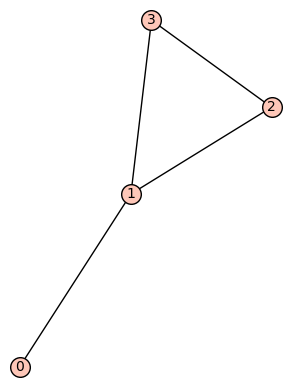
\includegraphics[width=\textwidth]{unorderedvertices}
		\caption{Edges treated as unordered pairs of vertices}
		\label{fig:unorderedvertices}
	\end{subfigure}
	\hfill
	\begin{subfigure}[b]{0.4\textwidth}
		\centering
		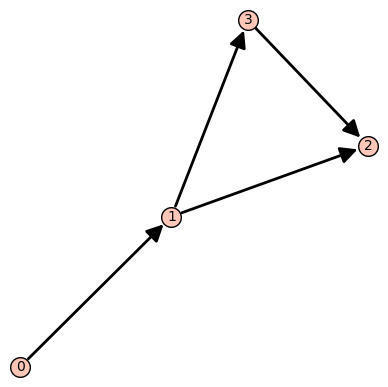
\includegraphics[width=\textwidth]{orderedvertices}
		\caption{Edges treated as ordered pairs of vertices}
		\label{fig:orderedvertices}
	\end{subfigure}
	\caption{Difference between a graph and a digraph.}
	\label{fig:directedvsnotdirected}
\end{figure}

We will continue giving some basic definitions for digraphs. They usually are only extensions of the corresponding definitions for graphs; therefore, we could define again all the concepts given for graphs, but we shall only present the most important for our needs.\\

\subsection{The Underlying Graph}
As we can see in Fig. \ref{fig:directedvsnotdirected}, we can obtain a graph from a digraph \cite{wilsonwatkins}.

\begin{defn}
	Let \textit{D} be a digraph. The \textit{underlying graph} of \textit{D} is the graph \textit{G} obtained by replacing each directed edge by the corresponding undirected edge. We say that \textit{D} is an orientation of \textit{G} called an \textit{oriented graph}. In the same way we can obtain an \textit{oriented graph} \textit{D} from a graph \textit{G} by choosing an orientation for each edge.
\end{defn}

\subsection{Subdigraphs}
We can also construct the subdigraphs of a digraph \textit{D} \cite{wilsonwatkins}:

\begin{defn}
	Let \textit{D} be a digraph with vertex-set $V(D)$ and edge set $E(D)$. A \textit{subdigraph} of $D$ is a digraph all whose vertices belong to $V(D)$ and all whose directed edges belong to $E(D)$.
\end{defn}

An example of a digraph and a subdigraph is shown in Fig. \ref{fig:subdigraphs}.

\begin{figure}[h]
	\centering
	\begin{subfigure}[b]{0.4\textwidth}
		\centering
		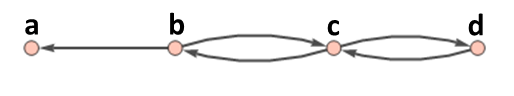
\includegraphics[width=\textwidth]{subdigraph_a}
		\caption{$D=(V(D),E(D))$ where\\   $V=\{a,b,c,d\}$ and $E=\{ba,bc,cb,cd,dc\}$}
		\label{fig:subdigraph_a}
	\end{subfigure}
	\hfill
	\begin{subfigure}[b]{0.4\textwidth}
		\centering
		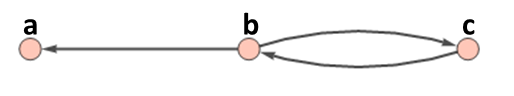
\includegraphics[width=\textwidth]{subdigraph_b}
		\caption{$C=(V(C),E(C))$ where\\   $V=\{a,b,c\}$ and\\$E=\{ba,bc,cb\}$}
		\label{fig:subdigraph_b}
	\end{subfigure}
	\caption[A subdigraph.]{(b) is a subdigraph of (a).}
	\label{fig:subdigraphs}
\end{figure}

\subsection{Local Degrees in a Digraph}
In Definition \ref{degree}, we saw that we can regard the degree of a vertex as the number of lines or edges connected to it, counting by two if the corresponding edge is a loop.
Due to the nature of digraphs, we can consider two distinct types of degrees depending in if the edge is going in or going out of the vertex, i.e., we have two local degrees \cite{douglas}:

\begin{defn}
	Let \textit{v} be a vertex in a directed graph. The \textit{vertex out-degree} $ d^{+} (v) $ of \textit{v} is the number of outgoing directed edges from it, that is, the number of edges with tail \textit{v}. The \textit{vertex in-degree} $ d^{-} (v) $ of \textit{v} is the number of incoming directed edges from it, that is, the number of edges with head \textit{v}.
\end{defn}

For instance, for the digraph in Fig. \ref{fig:orderedvertices}, the in and out degrees of the vertices are: $ \{ d^{-} (0)=0 ,  d^{-} (1)=1 , d^{-} (2)=2 , d^{-} (3)=1 \} $ and $ \{ d^{+} (0)=1 ,  d^{+} (1)=2 , d^{+} (2)= 0, d^{+} (3)=1 \} $.
It must be noted that if a vertex in a digraph has a loop, this will contribute by one to the count of both degrees, the \textit{vertex out-degree} and the \textit{vertex in-degree}.

\subsection{Adjacency and Incidence Matrices for a Digraph}
We will define the adjacency matrix for the most general type of digraph, that is a digraph that can have multiple edges and loops (a multidigraph) but we will continue referring to them just as digraphs. We define \cite{wilsonwatkins}:

\begin{defn}
	Let \textit{D} be a digraph with \textit{n} vertices labeled $1,2,3,...,n$. The \textit{adjacency matrix A(D)} is the $n \times n$ matrix in which the entry in row \textit{i} and column \textit{j} is the number of directed edges going from vertex \textit{i} to vertex \textit{j}. 
\end{defn}

If we sum the row(column) elements of \textit{A(D)} for a given row(column) we will obtain the out-degree(in-degree) of the corresponding vertex. This property is very useful, and in fact, we will make use of it in the next chapters to compute random digraphs with a given in-degree.\\

Let \textit{v} and \textit{w} be vertices of a digraph. If \textit{v} and \textit{w} are joined by a directed edge, then \textit{v} and \textit{w} are said to be \textit{adjacent}. If the directed edge is directed from \textit{v} to \textit{w}, then the arc is said to be \textit{incident from v} and \textit{incident to w}. Then, the incidence matrix of a digraph is defined as follows \cite{wilsonwatkins}:

%\begin{defn}
	%Let \textit{D} be a digraph with \textit{n} vertices labeled $a,b,c,...,$ and m directed edges labeled $1,2,3,...,m$. The \textit{incidence matrix B(D)} is the $nXm$ matrix in which the entry in the row $b_{ij}$ is given by:
%Let \textit{D} be a digraph with \textit{n} vertices and m directed edges. The \textit{incidence matrix B(D)} is the $nXm$ matrix in which the entry in the row $b_{ij}$ is given by:
%	\[b_{ij} = \begin{cases}
%		1 & \text{if the directed edge j is incident from vertex i} \\
%		-1 & \text{if the directed edge j is incident to vertex i} \\
%		0 & otherwise \\
%		\end{cases}
%		\]
%\end{defn}
\begin{defn}
	%Let \textit{D} be a digraph with \textit{n} vertices labeled $a,b,c,...,$ and m directed edges labeled $1,2,3,...,m$. The \textit{incidence matrix B(D)} is the $nXm$ matrix in which the entry in the row $b_{ij}$ is given by:
Let \textit{D} be a digraph with \textit{n} vertices and m directed edges. The \textit{incidence matrix B(D)} is the $nXm$ matrix in which the entry in the row $b_{ij}$ is given by:
\begin{equation}	
	b_{ij} = \begin{cases}
		1 & \text{if the directed edge j is incident from vertex i} \\
		-1 & \text{if the directed edge j is incident to vertex i} \\
		0 & otherwise \\
		\end{cases}
\end{equation}
\end{defn}

An example of the adjacency and incidence matrices for a digraph is shown in Fig. \ref{fig:adj_inc_digraph}.
It can be noted, that the adjacency and incidence matrices of a digraph depend in the way we have labeled the vertices. Just as we did for graphs, we can use this fact to find isomorphic digraphs which we define next. %(which we define in the next section) by using permutations matrices to permute the rows and columns of the adjacency matrix in such a way that we are changing the order the vertices are labeled.

\begin{figure}[h]
\centering
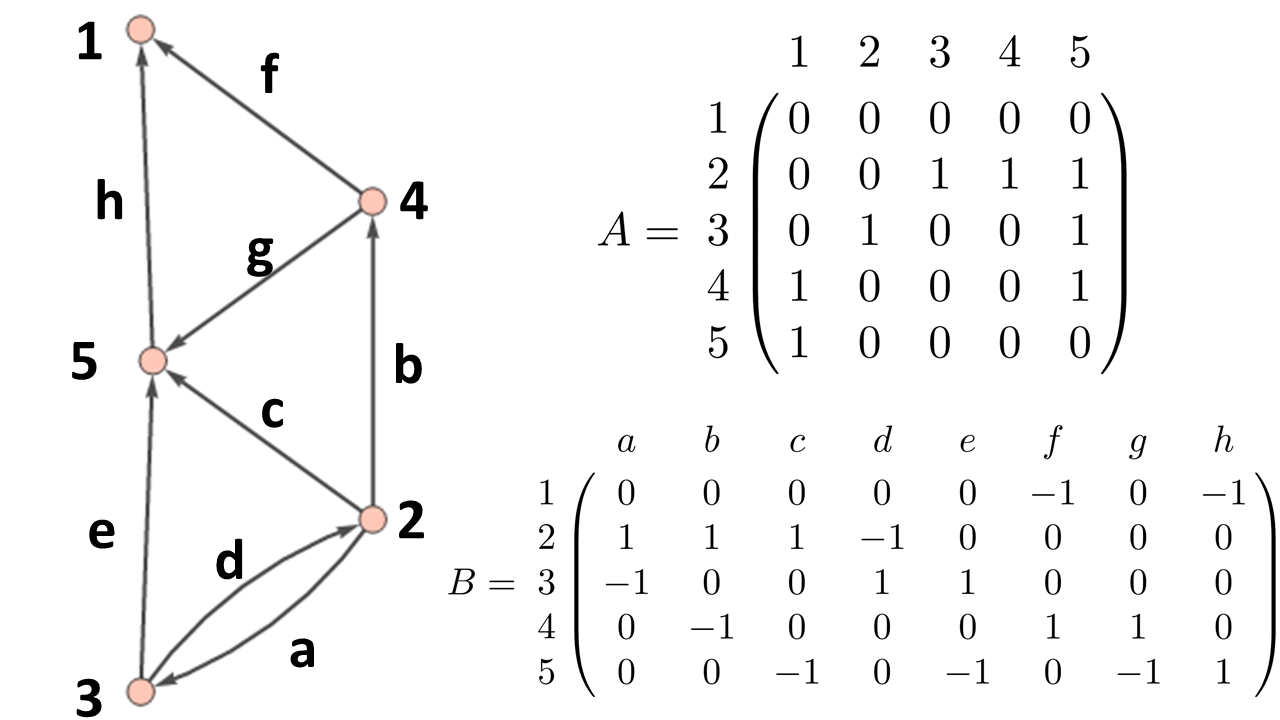
\includegraphics[width=\textwidth]{adj_inc_digraph}
\caption[Adjacency and incidence matrices for a digraph.]{An example digraph and its adjacency and incidence matrices labeled as $A$ and $B$ respectively.}
\label{fig:adj_inc_digraph}
\end{figure}

\subsection{Isomorphic Digraphs}
Another important concept we must extend for digraphs is the concept of isomorphism:

\begin{defn}
	Two digraphs $C$ and $D$ are \textit{isomorphic} if $D$ can be obtained from $C$ by relabeling the vertices- that is if there is a one-to-one correspondence between the vertices of $C$ and those of $D$, such that the number of edges joining any pair of vertices in $C$ is equal to the number of edges joining the corresponding pair of vertices (in the same direction) in $D$.
\end{defn}

Thus, we can ignore the labels of the vertices of digraphs in some applications, e.g., if we are checking if two digraphs are isomorphic or not, we can consider the corresponding unlabeled graphs, because we can relabel them as necessary (see Fig. \ref{fig:isomorphic_digraphs}).\\

\begin{figure}
	\centering
	\begin{subfigure}[b]{0.9\textwidth}
		\centering
		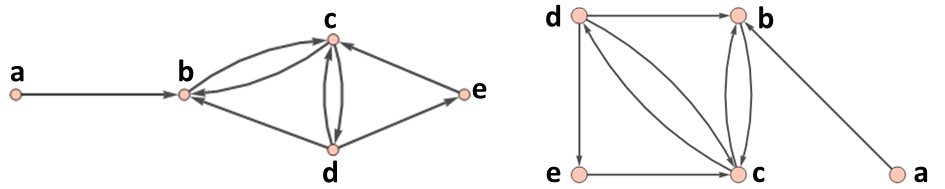
\includegraphics[width=\textwidth]{iso_digraph_a}
		\caption{}
		\label{fig:isodi1}
	\end{subfigure}
	\hfill
	\begin{subfigure}[b]{0.9\textwidth}
		\centering
		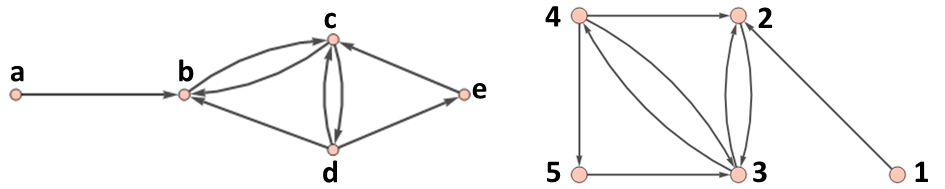
\includegraphics[width=\textwidth]{iso_digraph_b}
		\caption{}
		\label{fig:isodi2}
	\end{subfigure}
	\begin{subfigure}[b]{0.9\textwidth}
		\centering
		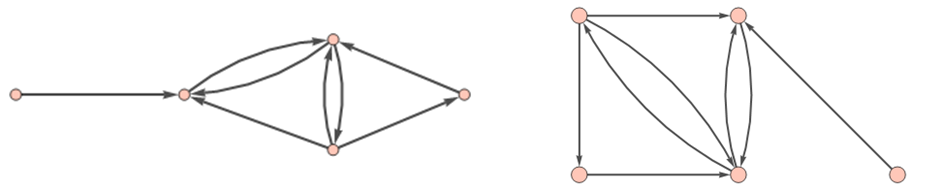
\includegraphics[width=\textwidth]{iso_digraph_c}
		\caption{}
		\label{fig:isodi3}
	\end{subfigure}
	\caption[Isomorphic digraphs.]{(a) Labeled digraphs that are the same. (b) Labeled digraphs that are not the same but are isomorphic. (c) Unlabeled digraphs that are isomorphic.}
	\label{fig:isomorphic_digraphs}
\end{figure}

As was said in Section \ref{isomorphic}, we can easily construct isomorphic digraphs in an analogous way to the one proposed for graphs by using permutations matrices to permute the rows and columns of the adjacency matrix in such a way that we are changing the order the vertices are labeled (see Fig. \ref{fig:iso_digraphs}). %We just must use permutation matrices to change the order in which the vertices had been labeled by means of permuting the rows and columns of the adjacency matrix of the digraph.

\begin{figure}[h]
\centering
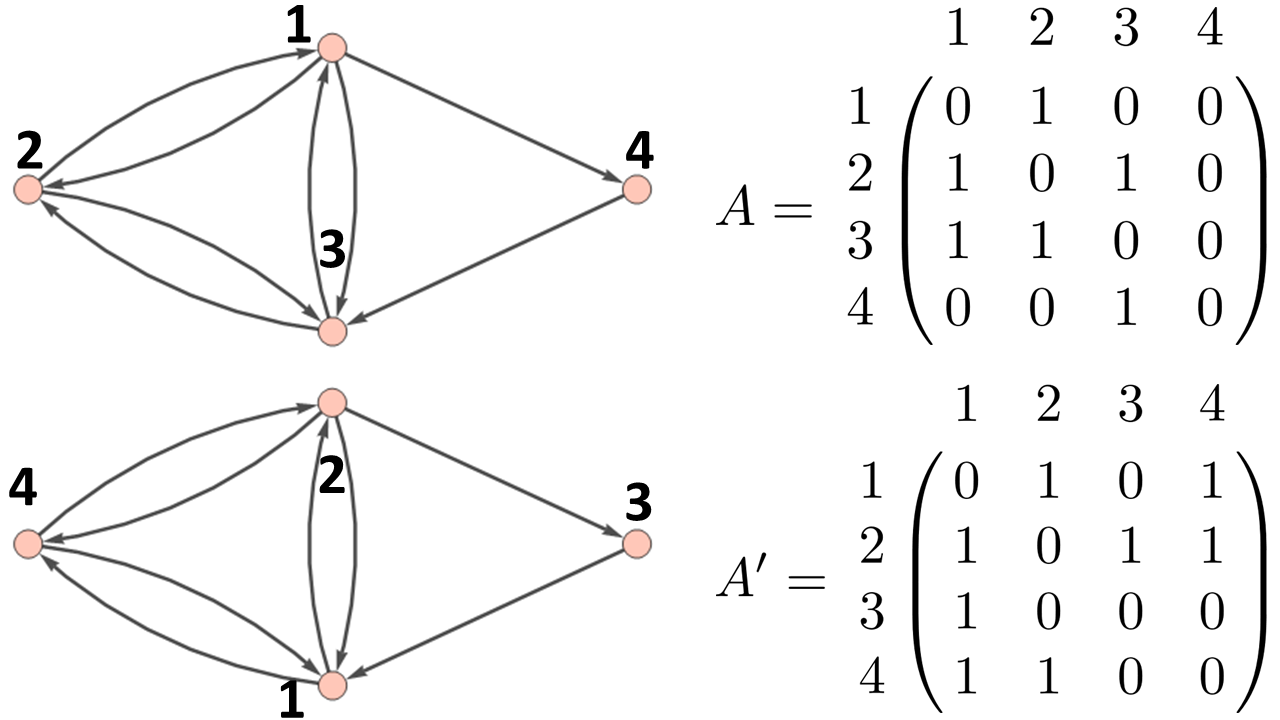
\includegraphics[width=\textwidth]{iso_digraphs}
\caption[Adjacency matrices for isomorphic digraphs.]{A digraph which vertices have been labeled in two different orders (they are isomorphic) and their corresponding adjacency matrices. The adjacency matrix $A'$ is obtained from $A$ by permuting the rows and columns of $A$ following the rules: $1 \mapsto 2$, $2 \mapsto 4$, $3 \mapsto 1$ and $4 \mapsto 3$}.
\label{fig:iso_digraphs}
\end{figure}

\subsection{Counting Digraphs}
As was said in Section \ref{count}, there are $ 2^{ \frac{1}{2} n(n-1) }$ simple labeled graphs with vertices $v_{1},...,v_{n}$. In the case of digraphs, there exist $2^{n^{2}}$ with these same vertices such that each ordered pair of them appears at most once as an edge. If we consider digraphs without loops and admit only one of the two possibilities $u \rightarrow v$ or $v \rightarrow u$ for each of them, then there are $ 3^{ \frac{1}{2} n(n-1) }$ different digraphs of this type \cite{douglas}.
%\subsubsection{Paths and Cycles in a Digraph}

%\section{Applications of Graphs}

\section{Random Graphs}
Sometimes, for some reasons, we will need to randomly create graphs that are different, but such that they all share some features in common. These features can be the number of vertices, edges, connections, etc. Thereby, we define a random graph as follows \cite{random_graphs}:

\begin{defn}
	A \textit{Random Graph} $G(n,p)$ is a probability space of all labeled graphs on $n$ vertices $\{1,...,n\}$, where for each pair $1 \leq i \leq j \leq n$, $ij$ is an edge of $G(n,p)$ with probability $p=p(n)$, independently of any other edges. Equivalently, the probability of a graph $G=(V,E)$ with $V=\{,1,...,n\}$ in $G(n,p)$ is $Pr[G]=p^{|E(G)|}(1-p)^{\binom{n}{2}-|E(G)|}$.
\end{defn}

Once the edge distribution is chosen, a random graph is obtained by picking out one graph within this distribution.
There have been proposed different edge distributions to attack different problems, following we will present some of them which we will use afterward, though strictly speaking they should be named pseudo-random graphs (see \cite{random_graphs} for a broader discussion).


\subsection{The Watts-Strogatz Small-World Graph Distribution}
\label{Watts-Strogatz}
This graph distribution is composed of graphs which are built using the following random procedure. We start with a circulant graph of $n$ vertices and jump list $\{1,2,...,k\}$. Then, we introduce disorder to this graph by rewiring each edge with a probability $p$, making sure that no loop or multiples edge is created. Evidently, $p$ satisfies $0 \leq p \leq 1$. For $p=0$ we have graphs which show regularity and order, meanwhile as we increase the value of $p$ we increase the disorder until we reach $p=1$ where the graph edges are totally disordered \cite{strogatz}. In Fig. \ref{fig:strogatz_graphs} three random graphs generated using this distribution by means of the built-in function \textit{WattsStrogatzGraphDistribution} of Mathematica are shown.

\begin{figure}[h]
\centering
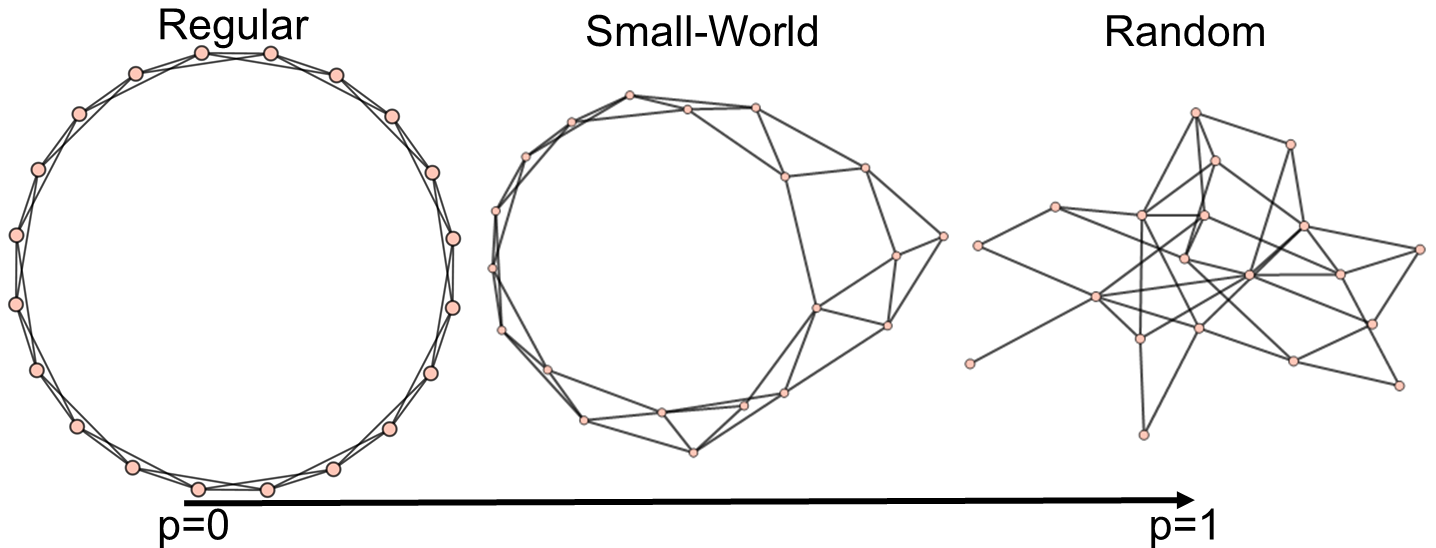
\includegraphics[width=\textwidth]{strogatz_graphs}
\caption[Three random graphs generated by using the Watts-Strogatz graph distribution.]{Three random graphs of $20$ nodes generated by using the Watts-Strogatz graph distribution with increasing $p$ value. The starting graph chosen was the circulant graph $Ci_{n} (1,2,3,4,)$, i.e., the complete graph $K_{4}$ as can be seen for $p=0$. The graphs like the middle one with regular lattices and small characteristic path lengths are known as "small-world" networks \cite{strogatz}.}
\label{fig:strogatz_graphs}
\end{figure}

\subsection{The Barabási-Albert Graph Distribution}
\label{Barabasi-Albert}
The graphs generated by this distribution are useful since they can describe networks of complex and possibly unknown topology such as the topology of web pages where nodes are individual web pages and the edges are the hyperlinks or the peer-reviewed scientific literature where the nodes are the publications and the edges are citations \cite{scale_free}. These graphs are also known as scale-free networks and their construction is based on preferential attachment since they expand by adding vertices which attach preferentially to high degree vertices. They have the property that the probability of a given vertex $v$ of having a vertex degree $d(v)$ decays as a power-law $P(d(v)) \sim d(v)^{-\gamma}$ where $\gamma>0$. The preferential connectivity is achieved with the following procedure \cite{albert}. Starting from a graph of $(n-m)$ vertices we add at each step a vertex with $k$ edges. These new $k$ edges are randomly attached to vertices at random with the probability of linking a node $v_{i}$ given by \cite{scale_free}:

\begin{equation}
\label{scale_free}
P(linking \, to \, node \, v_{i}) \sim \frac{d(v_{i})}{\sum_{j} d(v_{j})}
\end{equation}

This procedure is performed $m$ times, i.e., until we have a graph with $n$ vertices. In Fig. \ref{fig:albert_graphs} three random graphs generated using this distribution by means of the built-in function \textit{BarabasiAlbertGraphDistribution} of Mathematica are shown.

\begin{figure}[h]
\centering
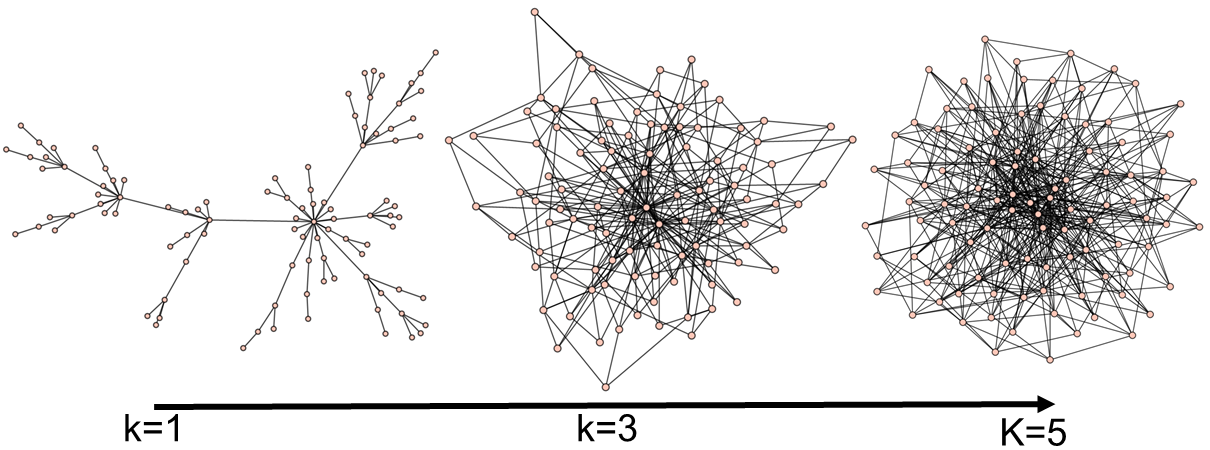
\includegraphics[width=\textwidth]{albert_graphs}
\caption[Three random graphs generated by using the Barabási-Albert graph distribution.]{Three random graphs of $100$ nodes generated by using the Barabási-Albert graph distribution. They were constructed starting from a cycle graph with $3$ vertices. At each step was added a vertex with $1,3$ and $5$ edges respectively.}
\label{fig:albert_graphs}
\end{figure}

\subsection{The Uniform Graph Distribution}
This is perhaps the simplest graph distribution. The sample space is made up just of all the simple graphs of $n$ vertices and $k$ edges. This graph distribution is implemented in Mathematica by means of the built-in function \textit{UniformGraphDistribution}. Alternatively, the sample space can consider all the directed graphs of $n$ vertices and $k$ directed edges, or even we can be more specific and consider all the directed graphs of $n$ nodes with vertex out-degree $ d^{+}$ and vertex in-degree $ d^{-}$.


\section{Other Ways of Representing Graphs}
\label{representations}
%Throughout this chapter, we have used different ways to represent a graph. For instance, we began describing a graph using lists, then we moved to matrices, even we could consider the graphical representations to describe graphs. To finish this chapter, it must be mentioned that in addition to the ones used here, there are many other ways to encode or represent a graph and they do not necessarily have to be new mathematical objects. For example, we could continue using lists, but instead of giving the list of vertices or edges of the graph, we could give a nested list with the list of vertices adjacent to each vertex in the graph which is known as the adjacency list. Another option could be to give a list with the vertex degree of each vertex in the graph. Or we could use other types of matrices, for example, we could use the \textit{Kirchoff Matrix} which we did not define here but it is only another way to encode a graph.
Throughout this chapter, we have used diverse ways to represent a graph. For instance, we began describing a graph using lists, then we moved to matrices, even we could consider the graphical representations as another type of representation. To finish this chapter, it must be mentioned that in addition to the ones used here, there are many other ways to encode or represent a graph. For instance, we could continue using lists, but instead of giving the list of vertices or edges of the graph, we could give a nested list with the list of vertices adjacent to each vertex in the graph, this is known as the adjacency list. Another option could be to give a list with the vertex degree of each vertex in the graph. Or we could use other types of matrix representations, for example, we could use the \textit{Laplacian Matrix} which we did not define here.

It must be remarked, that each representation, encodes or is focused on a feature or information of the graph, so when we work with graphs, we have to use the representation that best fits our needs for a particular application. The representation used will have to allow us to perform calculations without the loss of the information we care about. Often, the adjacency matrix will satisfy our requirements, but other times it will not.

